% !TEX root = main.tex
% !TEX encoding = UTF-8
% !TEX program = pdflatex

\section{Network Models}
    In this section we describe how we developed the algorithms to generate the synthetic networks and than the Facebook network.
    
    To develop this models, we decided to use \textbf{Python} because is an easy and very flexible language, in addition there are many libraries and documentation related to our topic.
    We chose to use the library \textit{NetworkX}~\cite{NetworkX} because this library have a very fast learning curve.
    
    We made the assumption that the population are fully mixed, as described in this paper \cite{witten2007simulations}, so the susceptible population have a fixed probability $\beta$ per unit time to get the disease from any infected neighbour. The set of neighbour of a vertex $v \in V$ is denoted with $N_G(v) = \{u_1, u_2, ..., u_i \}$, where $u_k,~k=1,...,i$, is adjacent to a given vertex \verb|v|.
    Then we need to define the fixed probability $\gamma$ per unit time that represent the probability to be recovered/immunised.
    With this parameter we can model the population susceptible, infected and recovered by a system of ordinary differential equation Eq.\ref{eq:diffEq} proposed in the paper~\cite{witten2007simulations}:
    
    \begin{equation}\label{eq:diffEq}
      \left\{\begin{matrix}
        \frac{\mathrm{d} s}{\mathrm{d} t} = -\beta si, & 
        \frac{\mathrm{d} i}{\mathrm{d} t} = \beta si - \gamma i,& 
        \frac{\mathrm{d} r}{\mathrm{d} t} = \gamma i
    \end{matrix}\right.
    \end{equation}
    where $s$,$i$,$r$ are respective the number of susceptible, infected and recovered person at that moment.
    Where s in not increasing, i is not decreasing and the last equation is redundant since $(d/dt)(s + i + r) = 0$ implies that $s + i + r = N$, with \verb|N| the total number of nodes of graph $|V| \in G$, at all times.
    
    \subsection{Random Network}
        In this section we will describe how we implemented the random network generator.
        
        \begin{lstlisting}[language=Python, frame=single]]
import networkx as nx

# population number
N = 1000

# probability p of any two sites being
    connected
P = 0.001

# create a network with random neighbour
def createRandomNetwork():
    # create a new Graph for our social
        network
    G = nx.Graph(name='RandomNetwork')
    
    # generate N nodes
    for i in range(N):
        G.add_node("node"+str(i), 
            state = sirv.SUSCEPTIBLE,
            dayOfInfection = -1)

    # generate random link
    for source in G:
        for possibleNeighbor in G:
            if(source != possibleNeighbor
                and random() < P):
                
                G.add_edge(source,
                    possibleNeighbor)
    return G
        \end{lstlisting}
        
        At the beginning we defined the number of nodes and the probability that a node have to establish a link with another node.
        Then, in the function \verb|createRandomNetwork| we define the nodes and we generate a random number and make a comparison with the threshold, the probability that that node establish a connection, and if the random number is lower than the threshold, we add that link to the graph \verb|G|.
        
        Because of the nature of random number, the nodes' degree distribution will follow the Poisson distribution, defined by the Eq.\ref{eq:poisson}.
        \begin{equation}\label{eq:poisson}
          p(k) \approx \frac{\lambda^ke^{-\lambda}}{k!}
        \end{equation}
        The parameter $\lambda = N P$, where $N = |V|$ and \verb|P| is the probability to establish a connection. So we can interact with P to decide the shape of this curve, as showed in Fig.\ref{fig:poissonDistribution}\cite{wiky-Poisson}.
        
        \begin{figure}[t]
            \centering
            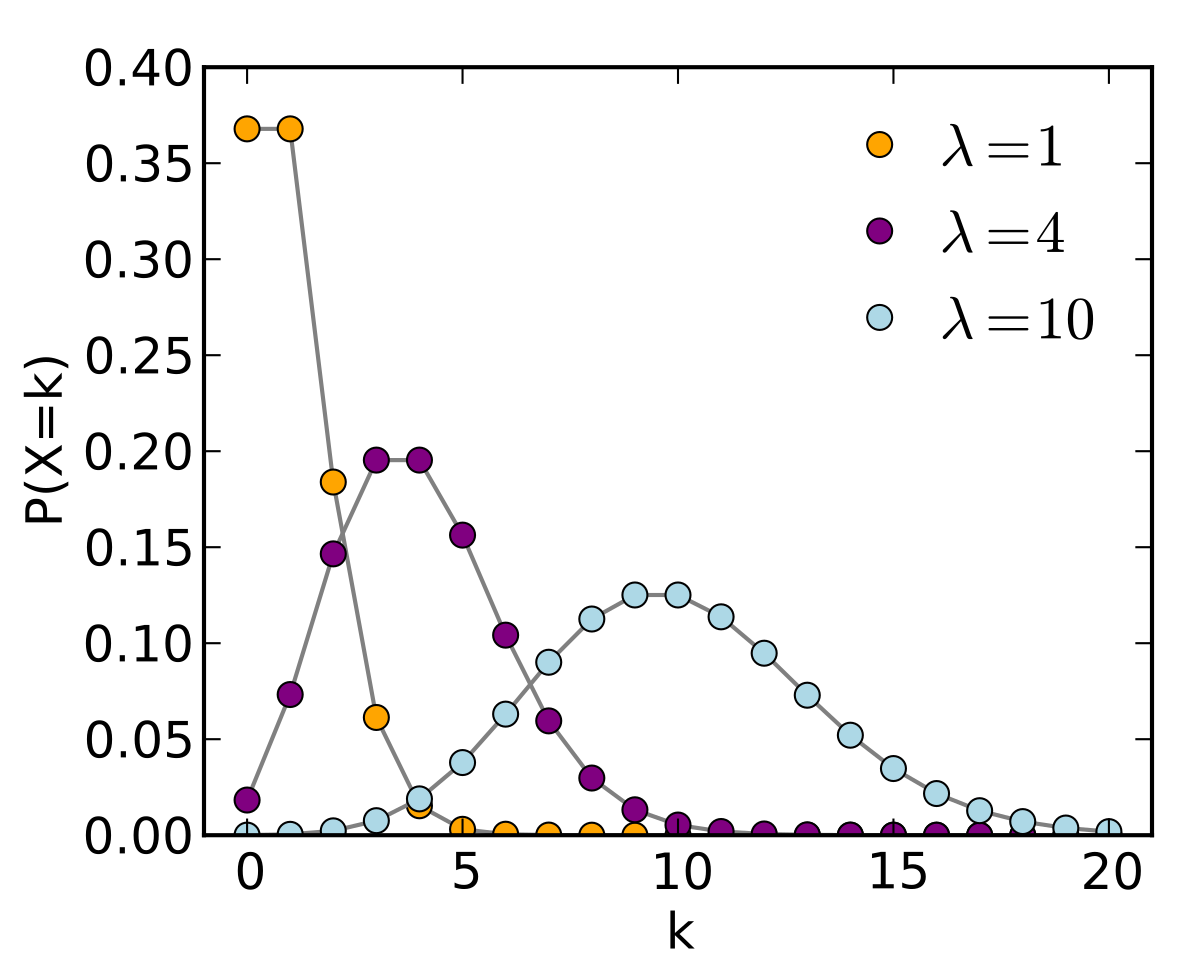
\includegraphics[width=\linewidth]{Figure/poissonDistribution.png}
            \caption{Poisson distribution graph}
            \label{fig:poissonDistribution}
        \end{figure}
        
    \subsection{Random Preferential Attachment}
        In this section we will describe how we implemented the random Preferential Attachment network generator.
        
        \begin{lstlisting}[language=Python, frame=single]]
import networkx as nx

# population number
N = 1000

# R0 basic reproduction number R0 in the 
    epidemic stage was estimated as 
    R0 = 1.5
R0 = 1.5
# fixed probability gamma per unit time 
    of any infected becoming removed
GAMMA = 0.267
# fixed probability beta per unit time 
    of contracting the disease from any
    infected in the population
BETA = R0 * GAMMA

def createPreferencialAttachmentN(a,m):
    # create a new Graph for our social
        network
    G = nx.Graph(
        name="PreferencialAttachmentN")
    for i in range(N):
        G.add_node("node"+str(i),
            state = sirv.SUSCEPTIBLE,
            dayOfInfection = -1)
    for source in G:
        k0 = G.degree[source]
        # print("possible N " + source)
        for possibleNeighbour in G:
            k = G.degree[source]
            y = 2 + ((k0/a)/m)
            pNode = beta(k + a, y)/
                    beta(k0 + a, y - 1)
            # print(pNode)
            if(source != possibleNeighbour
                and  random() < pNode):
                G.add_edge(source, 
                    possibleNeighbour)
    return G
        \end{lstlisting}
        
        In this case the probability to define if a node should establish a link or not is defined by the preferential attachment equation Eq.\ref{eq:prefAttach} \cite{wiky-prefAttach}.
        \begin{equation}\label{eq:prefAttach}
          P(k) = \frac{B(k+a,\gamma)}{B(K_0 + a, \gamma - 1)}
        \end{equation}
        
        for $k \geq k_0$ and zero otherwise, where $B(x,y)$ is the Euler beta function Eq.\ref{eq:euler}:
        \begin{equation}\label{eq:euler}
          B(x,y) = \frac{\Gamma(x)\Gamma(y)}{\Gamma(x+y)}
        \end{equation}
        
        with $\Gamma(x)$ is the standard gamma function, and $\gamma$ is defined as in the  Eq.\ref{eq:gamma}
        \begin{equation}\label{eq:gamma}
          B(x,y) = 2+ \frac{k_0+a}{m}
        \end{equation}
        where the constant $a > -k_0$ characterise the width of the curve and m is the number of link that will added, so this parameter influence the average nodes' degree, in other word the slope of our curve.
        
        This curve follows the Power law distribution, Fig.\ref{fig:PowerLaw}, in fact we have a very high pick in the left part of our graph and than a long tail in the right part of the graphic.
      
        \begin{figure}[t]
            \centering
            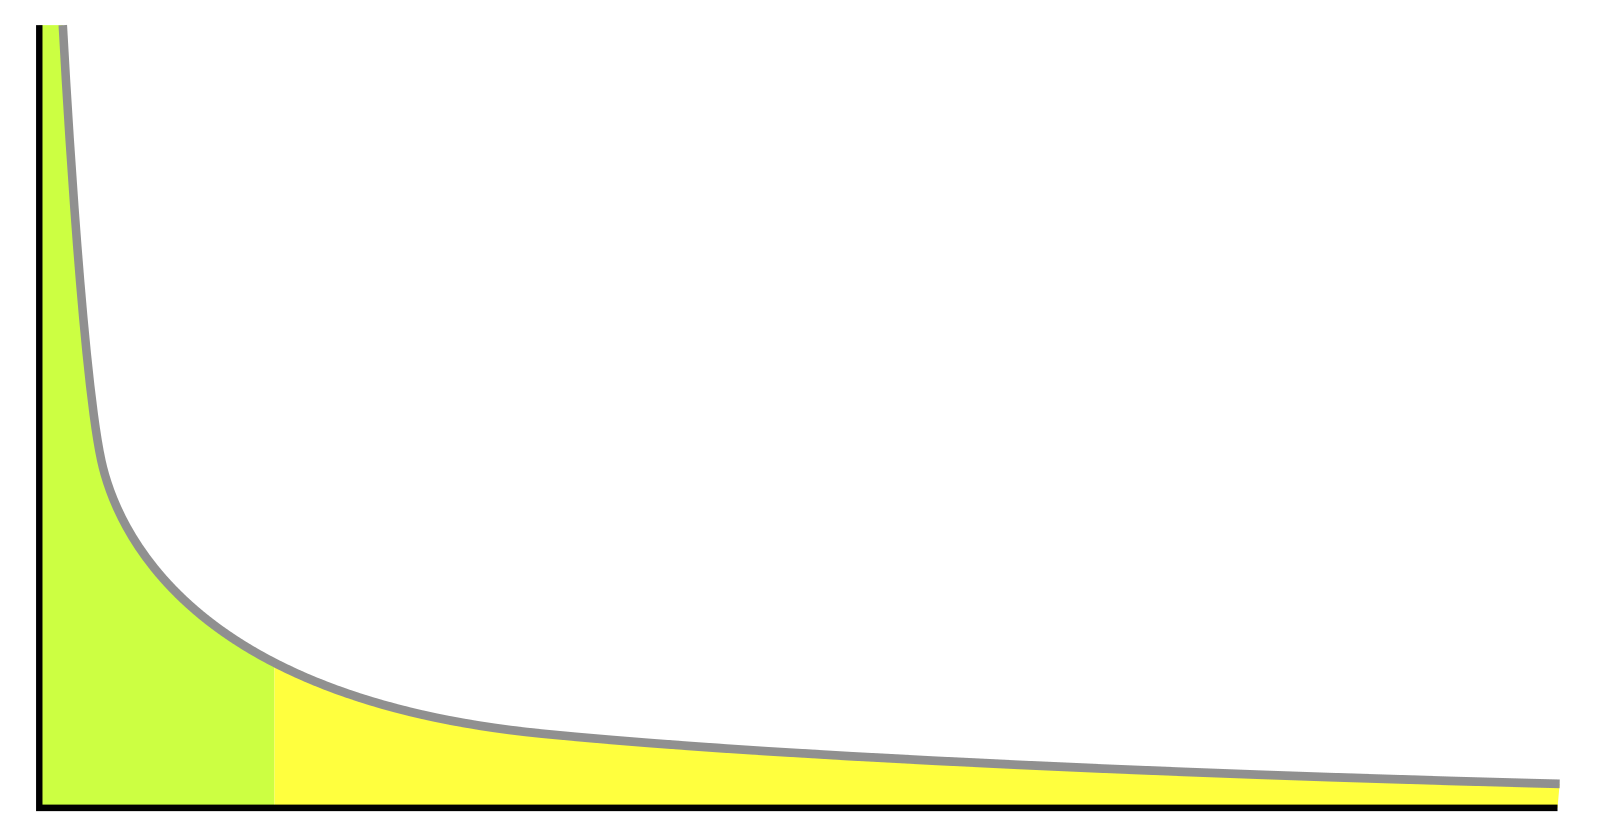
\includegraphics[width=\linewidth]{Figure/PowerLaw.png}
            \caption{Power law distribution graph}
            \label{fig:PowerLaw}
        \end{figure}
        
        After compute the percentage we evaluate if a random number is bigger or not in order to define if the link will be added or not.
        
    \subsection{Real Facebook Network}
        We imported the links of a real network based on Facebook. This data are collected by the Stanford University with the project SNAP \cite{stanford_Facebook}.
        
        This network is composed by 4039 Nodes and 88234 edges. Is possible see the shape of this network in the Fig.\ref{fig:Facebook}.
        \begin{figure}[t]
            \centering
            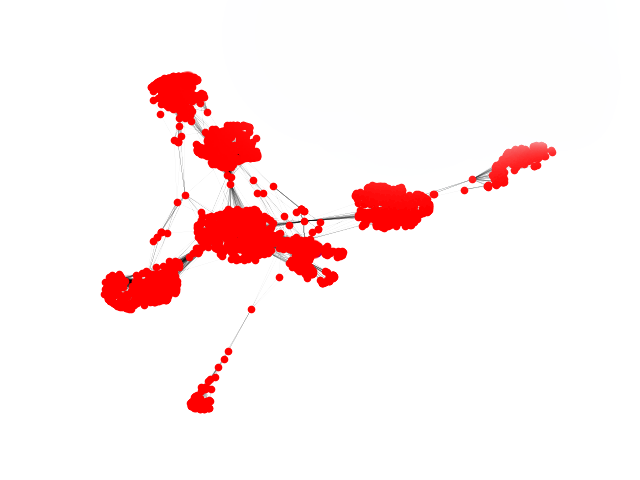
\includegraphics[width=\linewidth]{Figure/FacebookGraph.png}
            \caption{Facebook network graph}
            \label{fig:Facebook}
        \end{figure}
        
    \subsection{How the disease spread}
        In this section we are going to describe how we implements the spread of a disease.
        
        First of all we initialise all nodes by the following function: 
        
        \begin{lstlisting}[language=Python, frame=single]]
def infection(node, infectionProbability):
    if(random() < infectionProbability):
        G.node[node]['state'] = 
            sirv.INFECTED
        G.node[node]['dayOfInfection'] = 
            day
        \end{lstlisting}
        
        So, given a random number if this is smaller than a fixed probability than that node become infected and we save the day of this event.
        
        Than every node have a probability to become infected that is proportional to how many infected neighbour have a node and how many days its in touch with them.
        The probability of a susceptible node $n_s$ to became infected is:
        
        \begin{equation}
            p(n_s) = \sum_{d=1}^{d_{infected}}{\sum_{m = 0}^{k_{nd}}{\beta * (d - m_d)}}
        \end{equation}
        where $d_{infected}$ is the day that the node $n_s$ need to became infected, $d$ is the current day, $k_{nd}$ is the number of infected neighbour of n at the day $d$, $\beta$ in a fixed probability on a node to became infected in our case we fixed $\beta=0.01$, than $d$ is the current day and $m_d$ is the day that the node $m$ was infected.
        
        Symmetrically, to calculate the probability that an infected node $n_i$ have to recover is:
        
        \begin{equation}
            p(n_i) = \sum_{d=n_d}^{d_{recovered}}{\gamma * (d - n_d)}
        \end{equation}
        where $d_{recovered}$ is the day that the node $n_s$ pass form the state of infected to the state of recovered, $d$ is the current day, $n_d$ is the day that $n_i$ pass in the state of infected, $\gamma$ is the fixed probability to recover from the infection in our case it was fixed $\gamma=0.04$. 